\section{Use case 2: Monitoring electricity consumption}
\SectionPage

\begin{frame}
    \frametitle{Goals}
    \vspace*{\fill}
    Track the energy usage of a large campus, the \ac{BHC}, in Jette, using existing data collected over several years.

    \begin{columns}[onlytextwidth, c]
        \begin{column}{.47\textwidth}
            \textbf{General goals}:
            \begin{itemize}
                \item Having a global view on the data, centralized and well accessible for multiple user
                \item Minimizing the energy losses and overall consumption
                \item Identify where the exact sources of energy cost are
                \item Improve sustainability reducing energy need and peek request
            \end{itemize}
        \end{column}
        \begin{column}{.52\textwidth}
            \begin{figure}[ht]
                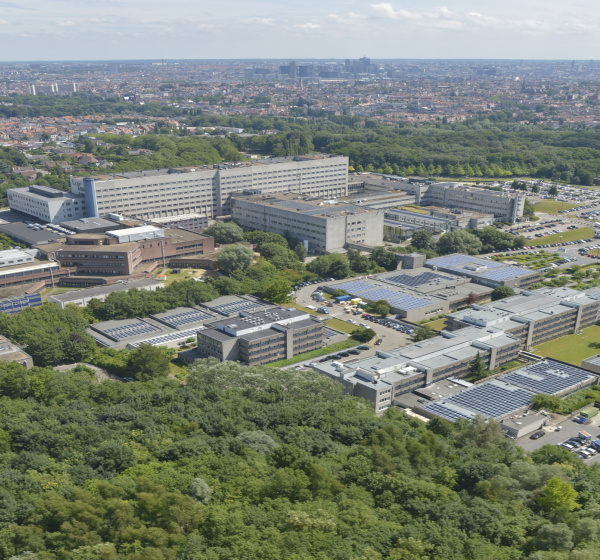
\includegraphics[width=0.78\textwidth]{frames/figures/jette_luchtfoto.jpg}
                \caption{\ac{BHC} aerial photo}
            \end{figure}
        \end{column}
    \end{columns}
    \vspace*{\fill}
\end{frame}

\begin{frame}
    \frametitle{Context}
    % We focus on the academic hospital distribution network, in closed-ring shape for increased reliability.
    \begin{figure}[ht]
        \fbox{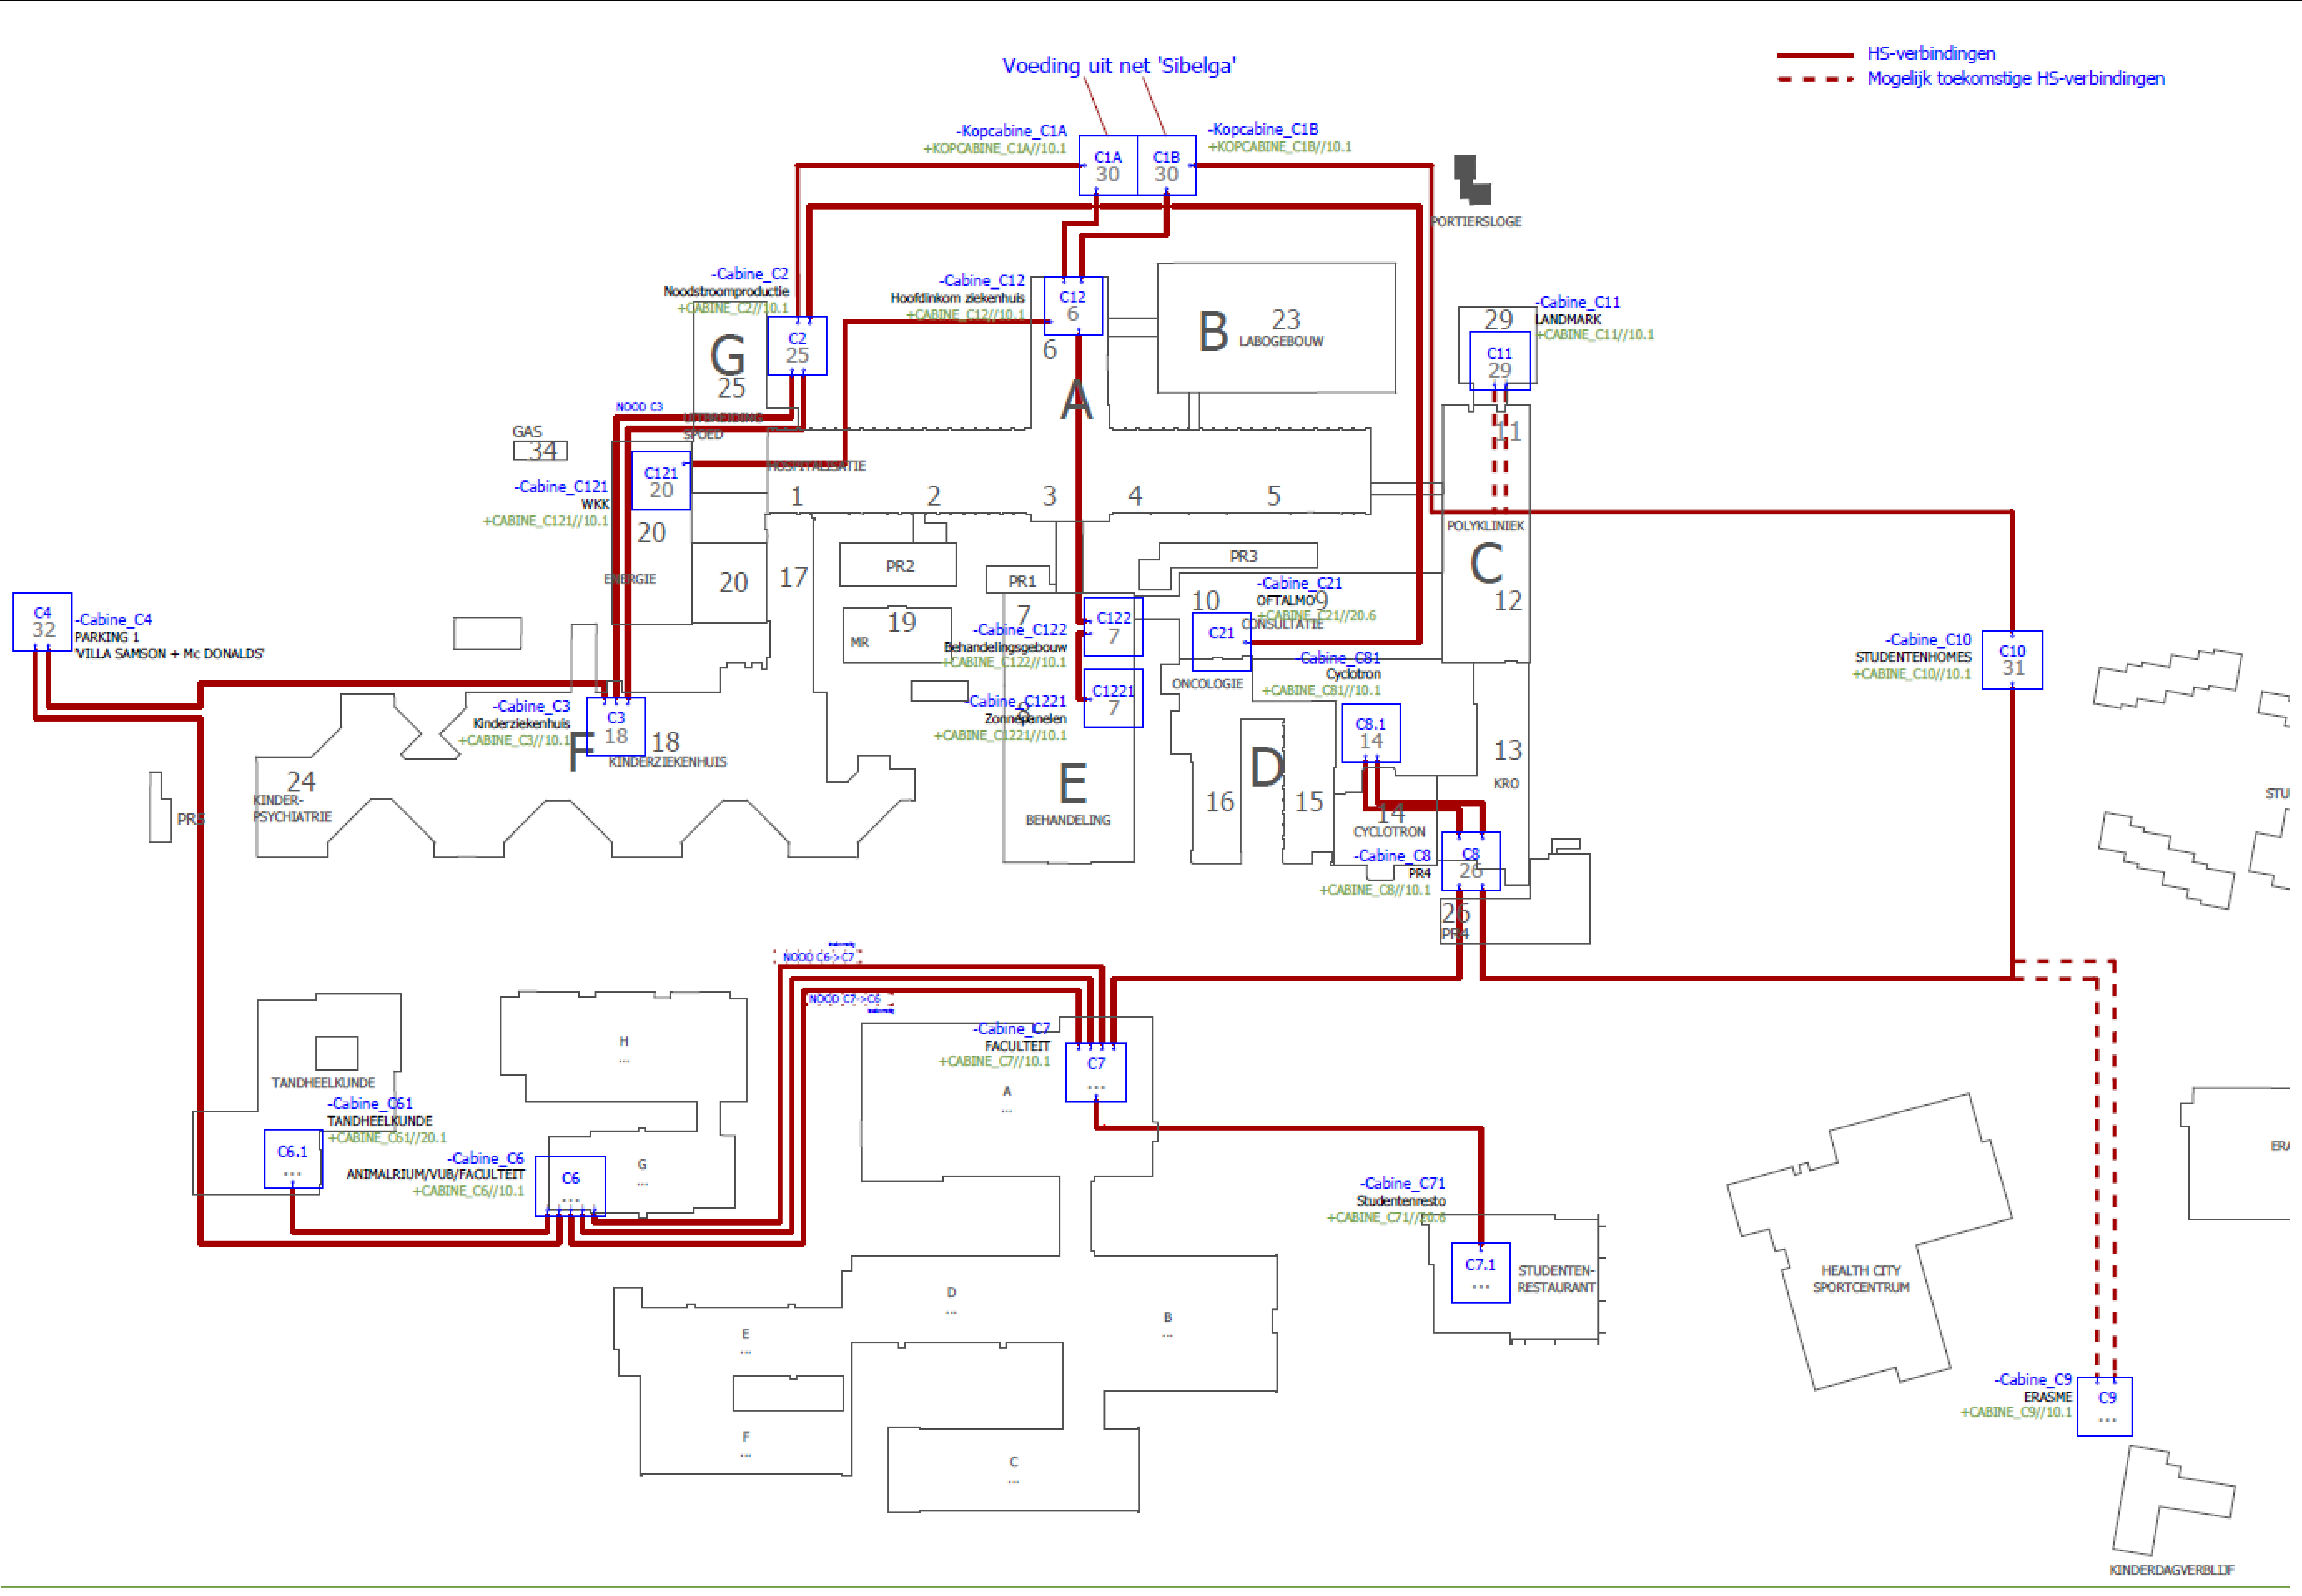
\includegraphics[width=0.78\textwidth]{vub/context/campus_site_layout.pdf}}
        \caption{\acs{UZB} electricity distribution network} %layout}
        \label{fig:bhc_site_layout}
    \end{figure}
\end{frame}

% \subsection{4 Phases}
\begin{frame}
    \frametitle{4 Phases -- I}
    \vspace*{\fill}
    \begin{columns}[onlytextwidth, c]
        \begin{column}{.47\textwidth}
            \begin{exampleblock}{Data sources}
                \begin{itemize}
                    \item Tries to reflect reality
                    \item Limited dataset
                    \item 15-minute ``electricity'' data
                    \item Also metedata source
                \end{itemize}
                Example:\\
                \texttt{root/NodeC3/Transformer\\
                    0302/ConsumerEnergy/\\
                    Bord\_Radiologie.csv}
            \end{exampleblock}
        \end{column}

        \begin{column}{.52\textwidth}
            \begin{figure}[ht]
                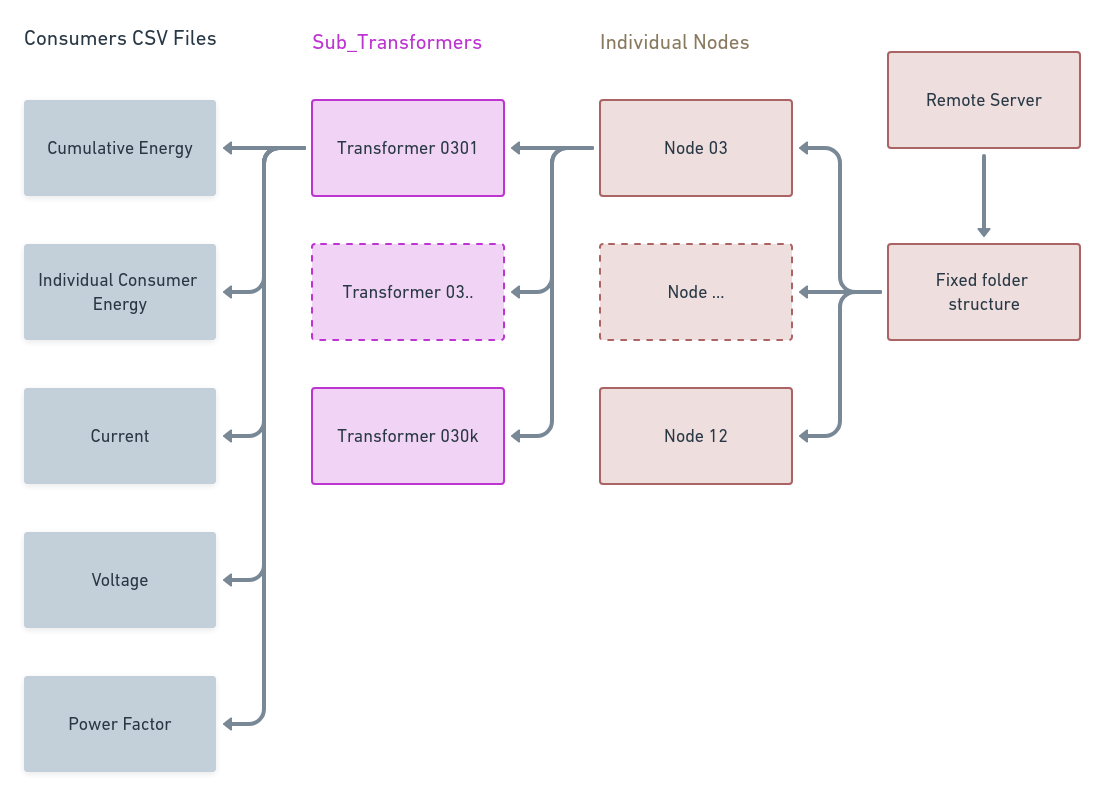
\includegraphics[width=\textwidth]{vub/flowcharts/folder_tree.png}
                \caption{\acs{VUB}'s folder tree structure}
            \end{figure}
        \end{column}
    \end{columns}
    \vspace*{\fill}
\end{frame}

\begin{frame}
    \frametitle{4 Phases -- II \& III}
    \vspace*{\fill}
    \begin{columns}[onlytextwidth, c]
        \begin{column}{.47\textwidth}
            \begin{exampleblock}{Commissioning}
                \begin{itemize}
                    \item \ac{SFTP}
                    \item automate remote access
                    \item automate ingestion
                \end{itemize}
            \end{exampleblock}
        \end{column}
        \begin{column}{.52\textwidth}
            \begin{exampleblock}{Data Management}
                \begin{itemize}
                    \item Multi processing script
                    \item Parsing, cleaning and tagging % w/ Pandas
                    \item Writing DB ``measurement''  %for each node
                \end{itemize}
            \end{exampleblock}
        \end{column}
    \end{columns}
    \begin{figure}[ht]
        \includegraphics[width=\textwidth]{vub/flowcharts/data-management.png}
        \caption{\acs{VUB}'s data ingestion flowchart}
    \end{figure}
    \vspace*{\fill}
\end{frame}

\begin{frame}
    \frametitle{4 Phases -- IV}
    \vspace*{\fill}
    \begin{columns}[onlytextwidth, c]
        \begin{column}{.47\textwidth}
            \begin{exampleblock}{Analysis}
                \begin{itemize}
                    \item[a]
                        \begin{itemize} % Basic visualisation
                            \item Variable n° of panels
                            \item Bottom: [V], [A], [PF]
                            \item Top: Cumulative [MWh]
                        \end{itemize}
                    \item[b]
                        \begin{itemize}
                            \item Usage statistics
                            \item Various $T$-period
                            \item \textit{Split-Apply-Combine} \& $\Delta$
                        \end{itemize}
                \end{itemize}
            \end{exampleblock}
        \end{column}
        \begin{column}{.52\textwidth}
            \begin{figure}[ht]
                \begin{subfigure}{\textwidth}
                    \centering
                    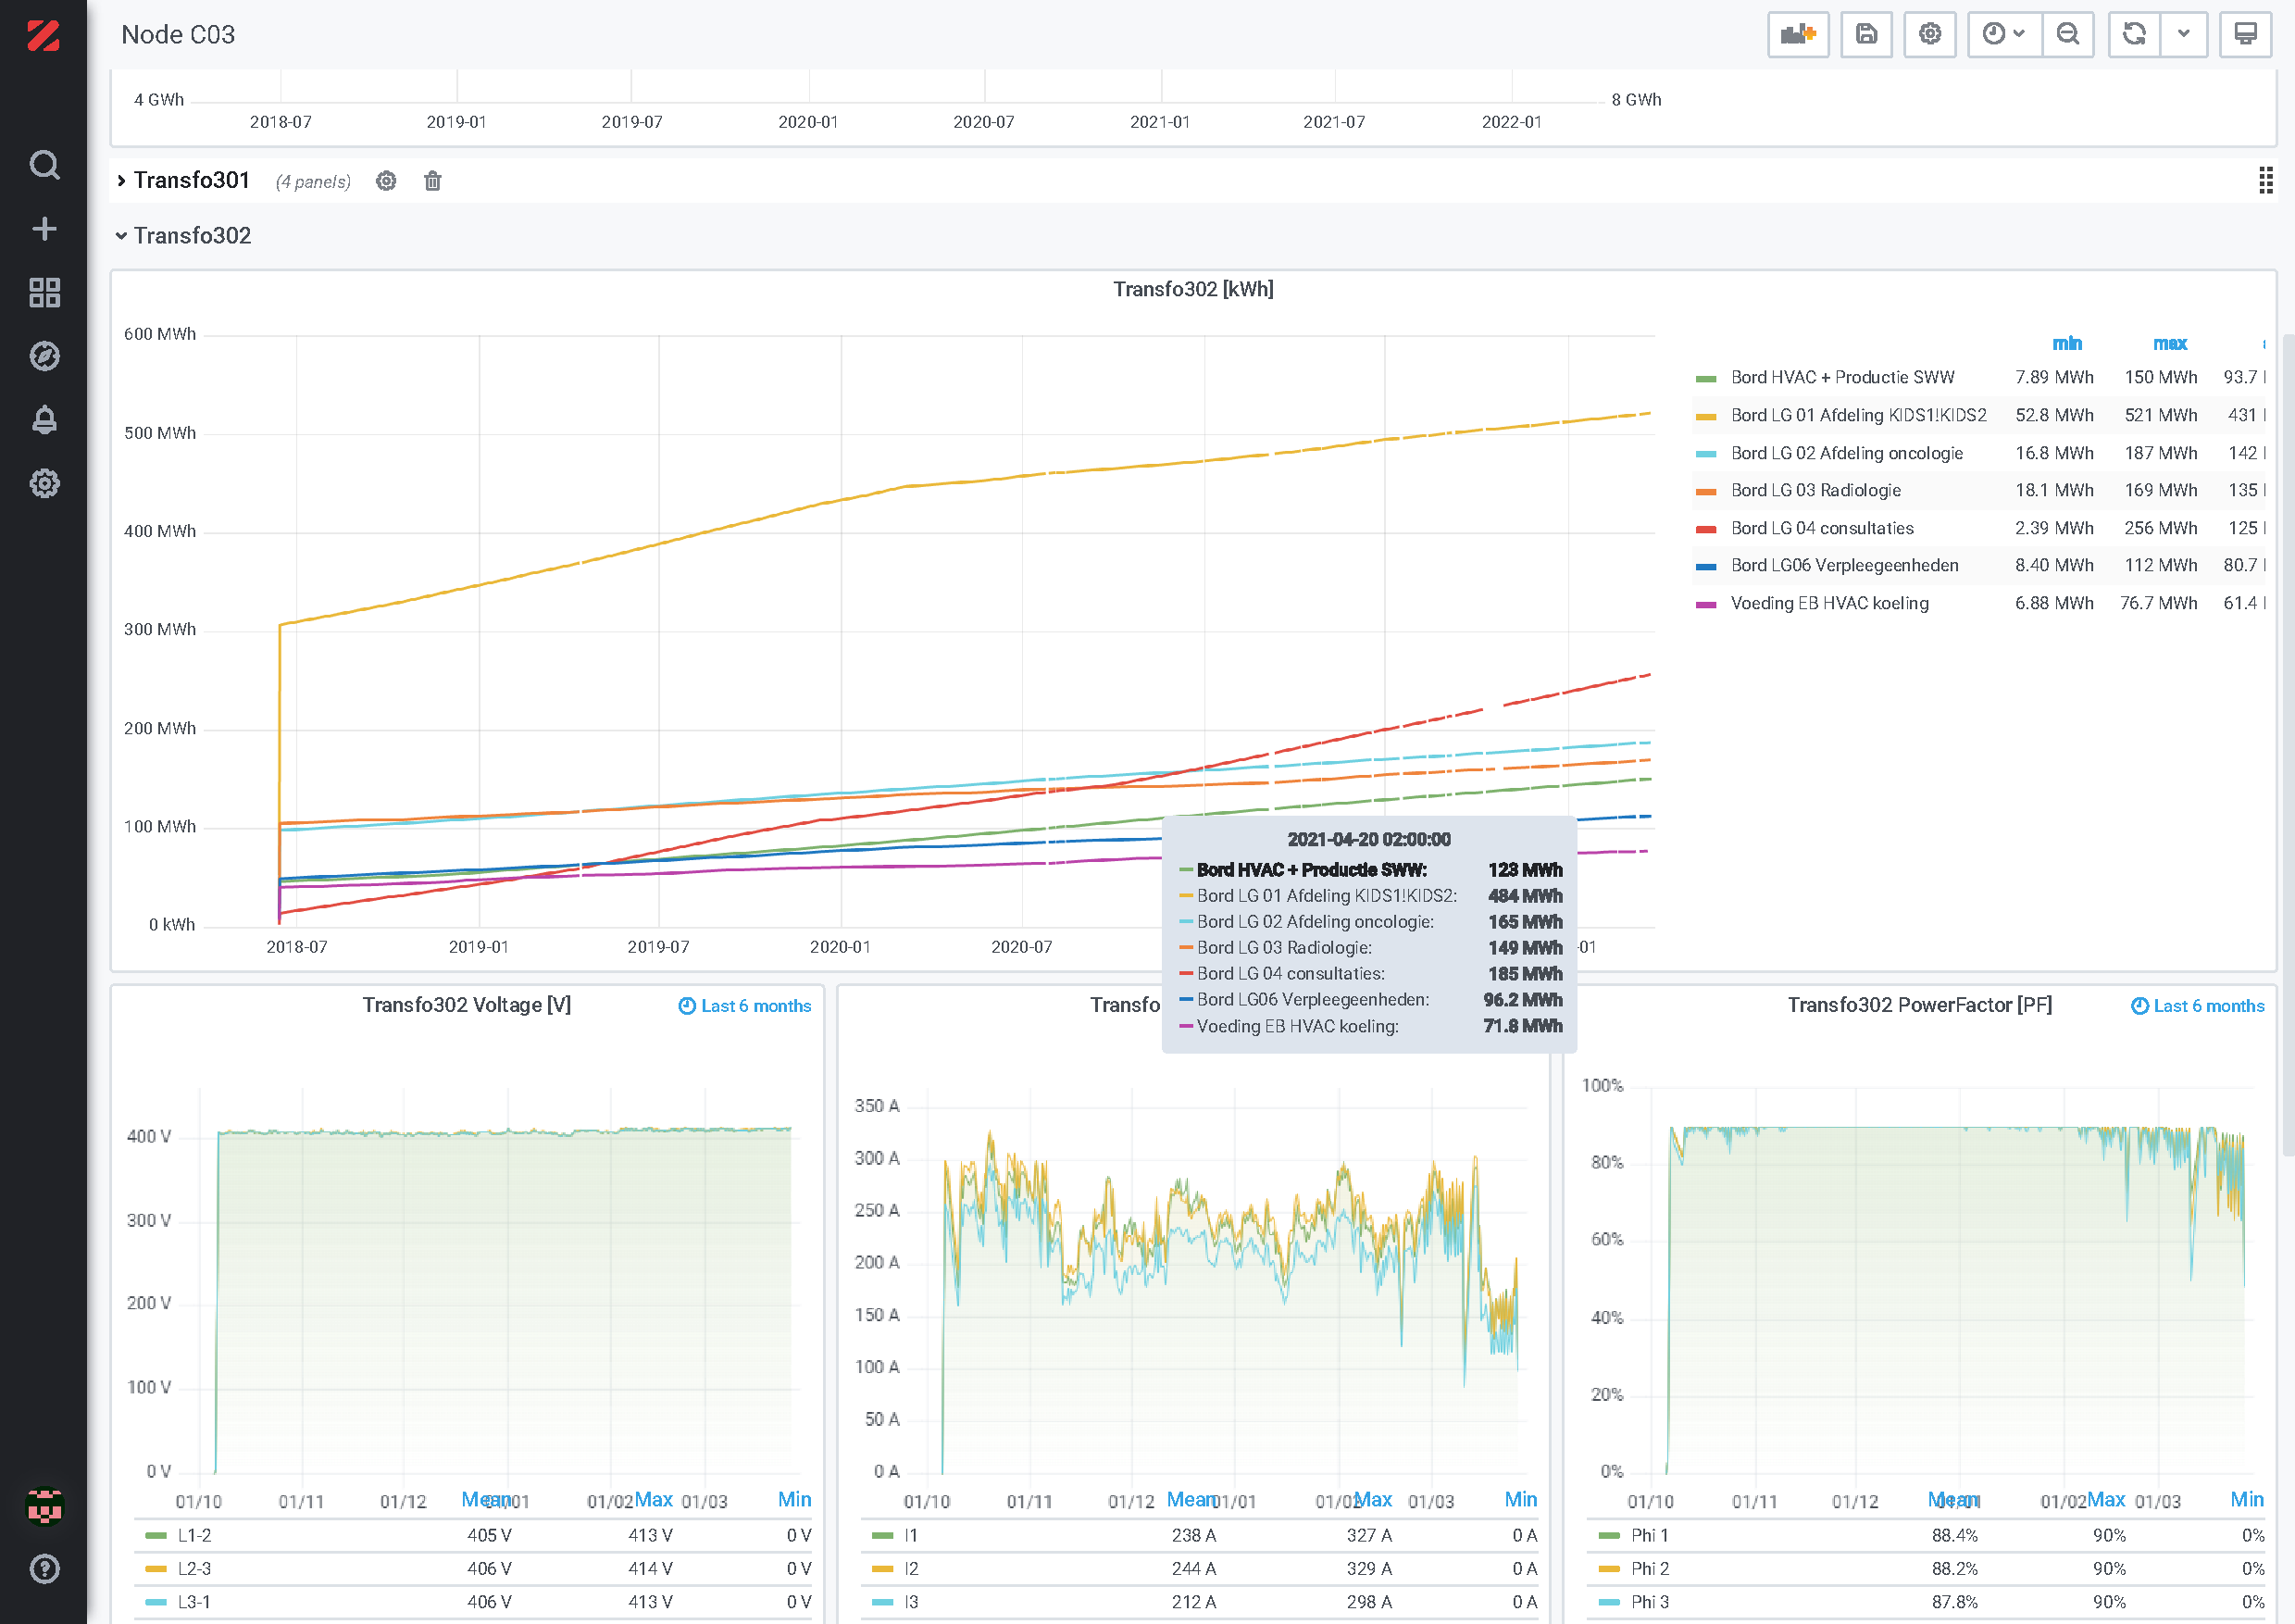
\includegraphics[clip, trim=0 0 0.1cm 3.5cm, width=0.87\textwidth]{vub/grafana/node_c03_transfo302_raw.pdf}
                    \caption{Transformer--302 raw data dashboard}
                \end{subfigure}
                \begin{subfigure}{\textwidth}
                    \centering
                    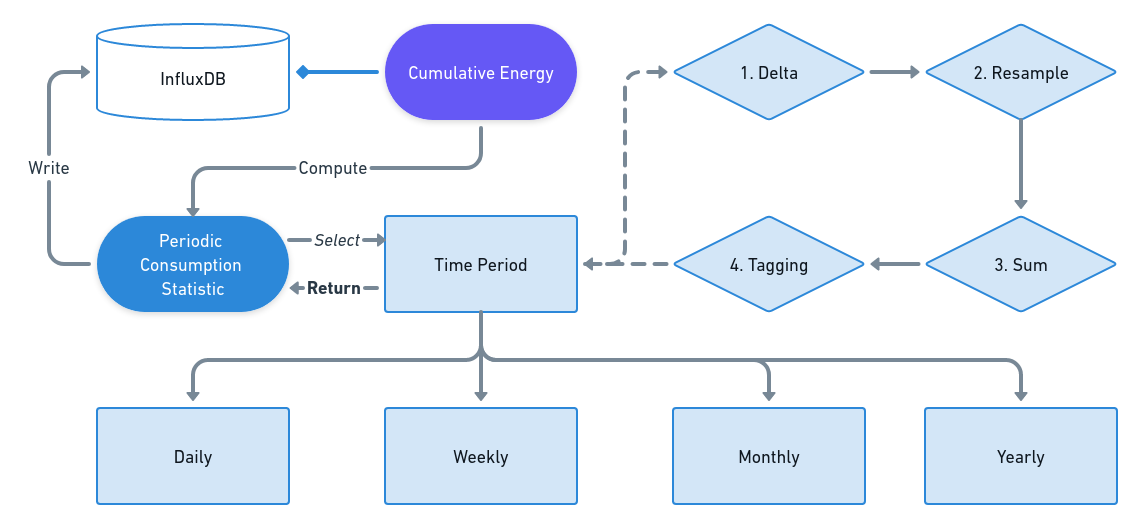
\includegraphics[width=0.87\textwidth]{vub/flowcharts/analystic_flowchart.png}
                    \caption{\acs{VUB}'s analytics chart}
                \end{subfigure}
            \end{figure}
        \end{column}
    \end{columns}
    \vspace*{\fill}
\end{frame}


\begin{frame}
    \frametitle{Results}
    \vspace*{\fill}
    Wide range of visualisation techniques: Bar plot, Pie chart, Status map.

    \begin{figure}
        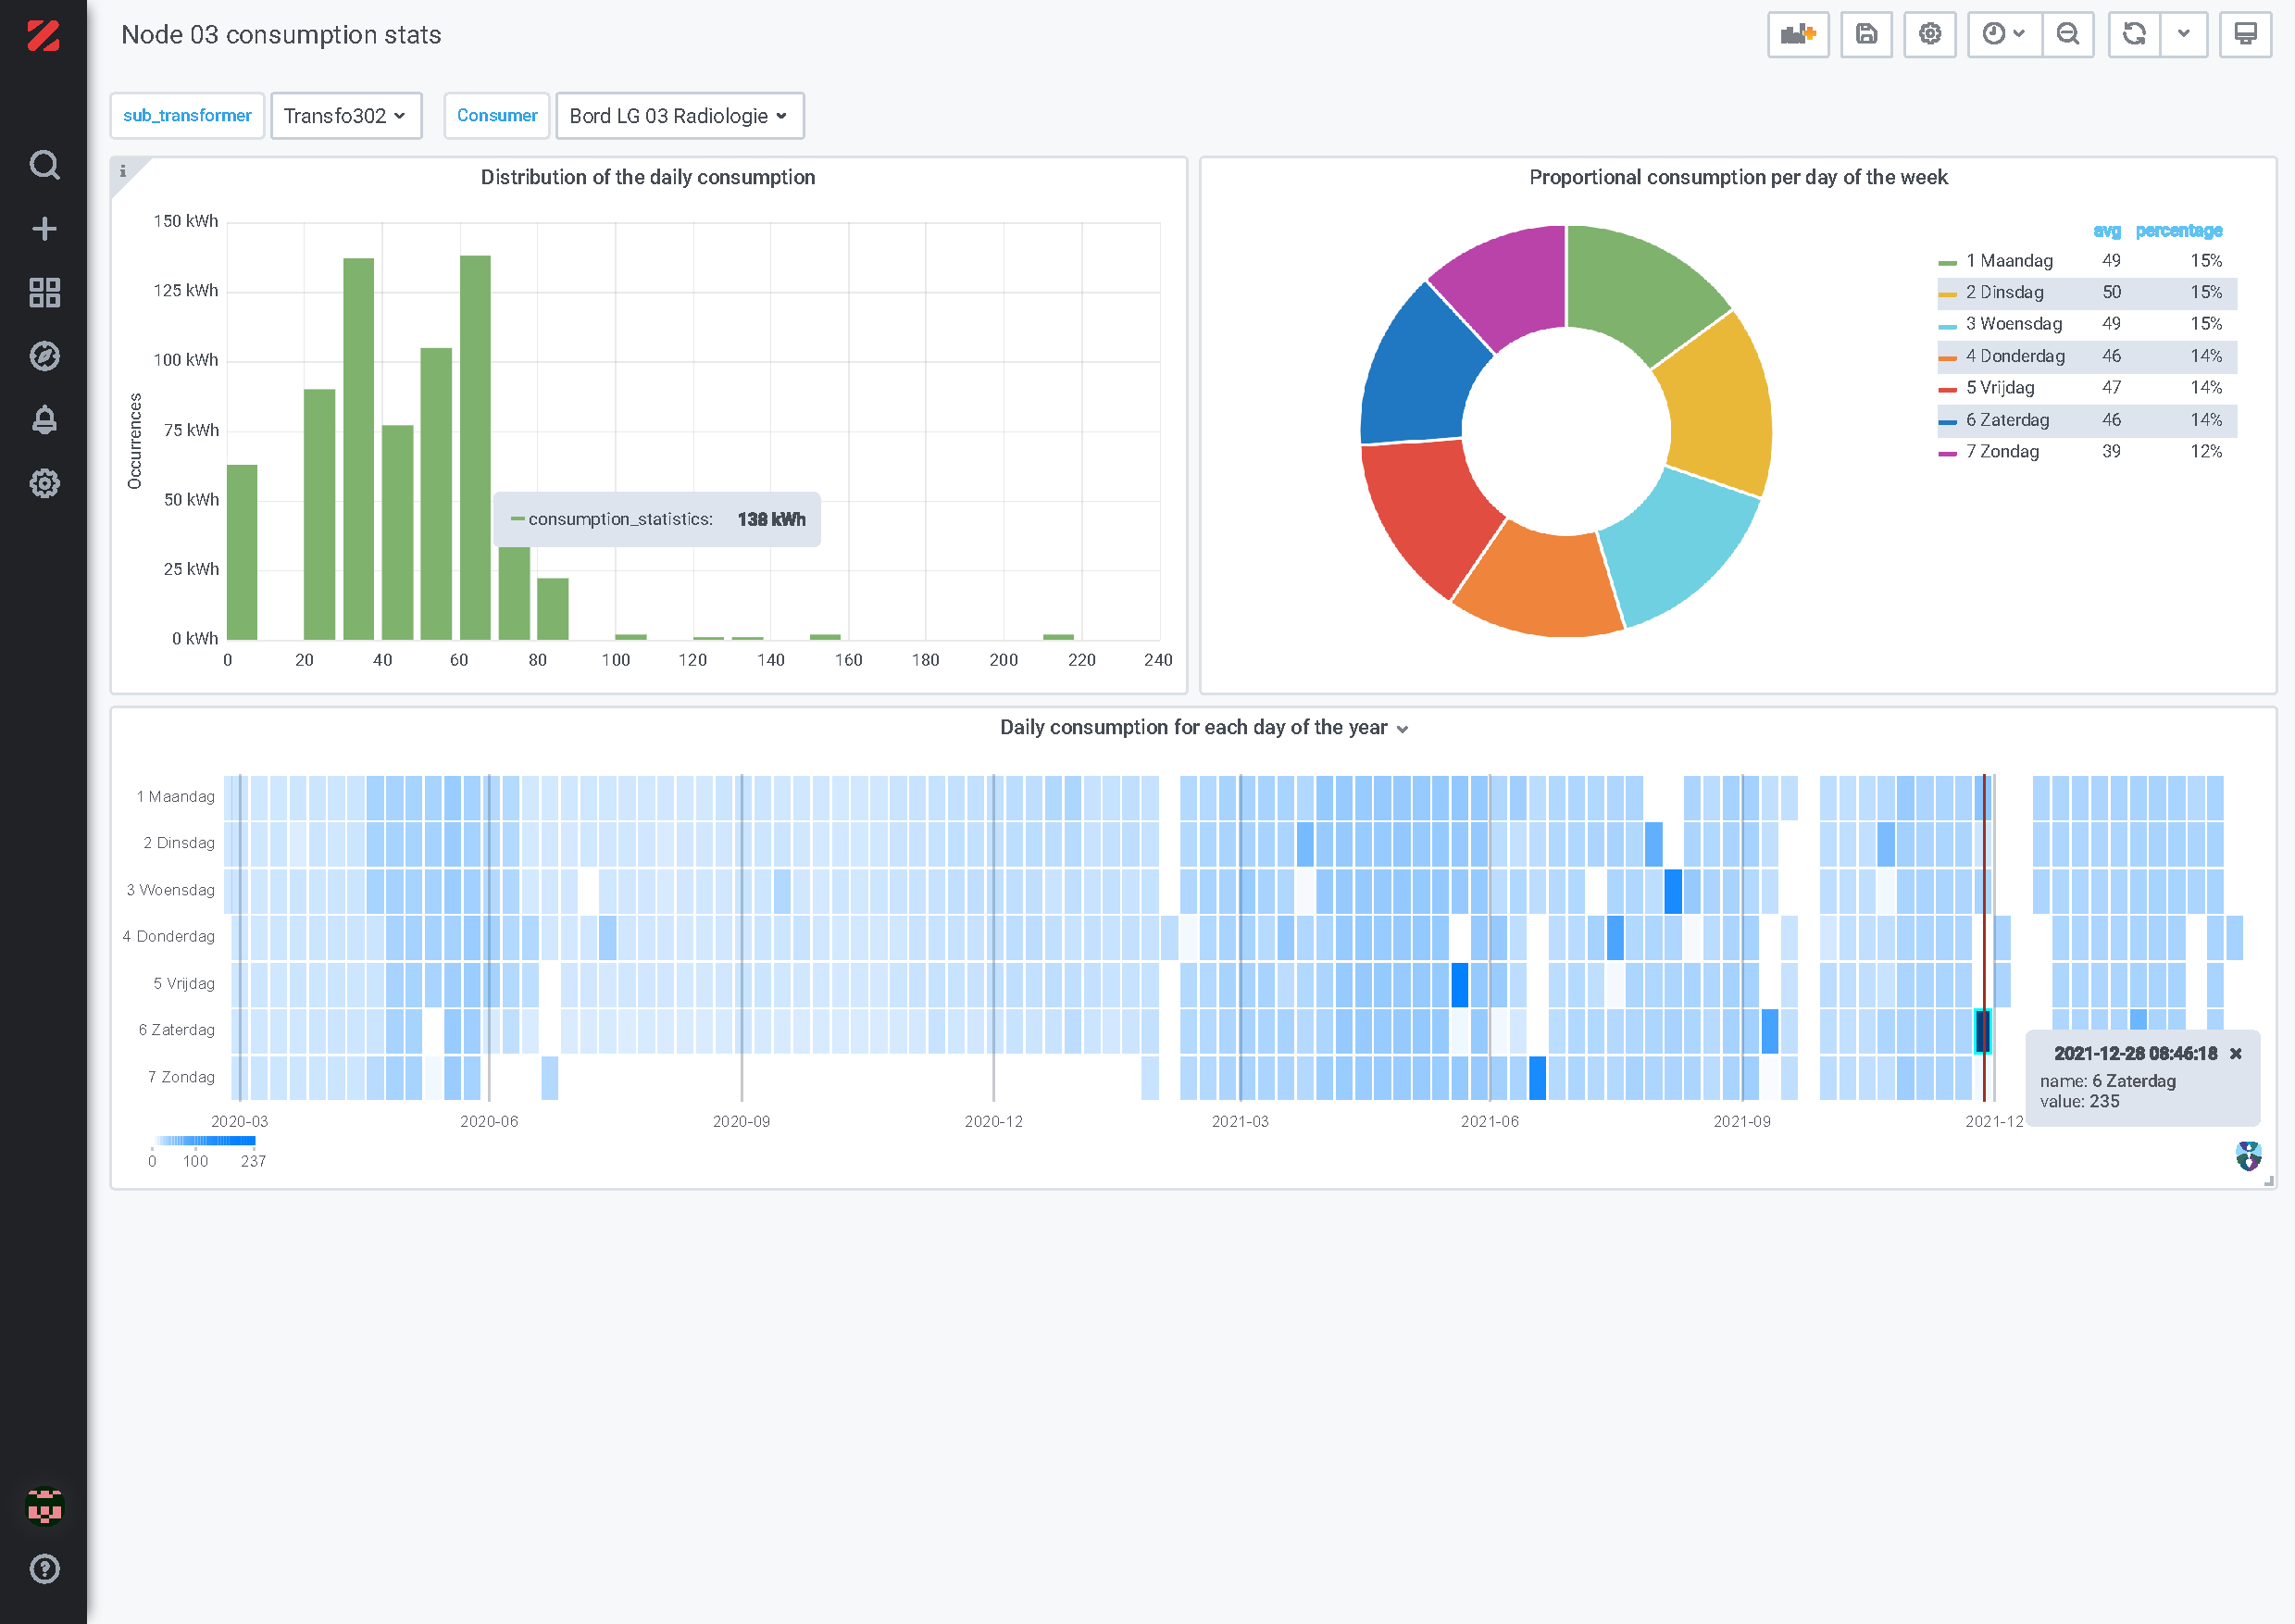
\includegraphics[clip, trim=0 7.5cm 0 0, width=.95\textwidth]{vub/grafana/node_c03_consumption_stats.pdf}
        \caption{Daily energy consumption of \acs{UZB} radiology ward}
    \end{figure}
    \vspace*{\fill}
\end{frame}

\begin{frame}
    \frametitle{Findings}
    \vspace*{\fill}
    
    VUB researchers were fairly satisfied with
    the project result, as they now are able to monitor most of the hospital
    consumption via dashboards, in detail, everywhere through a web browser.
    \begin{figure}[ht]
        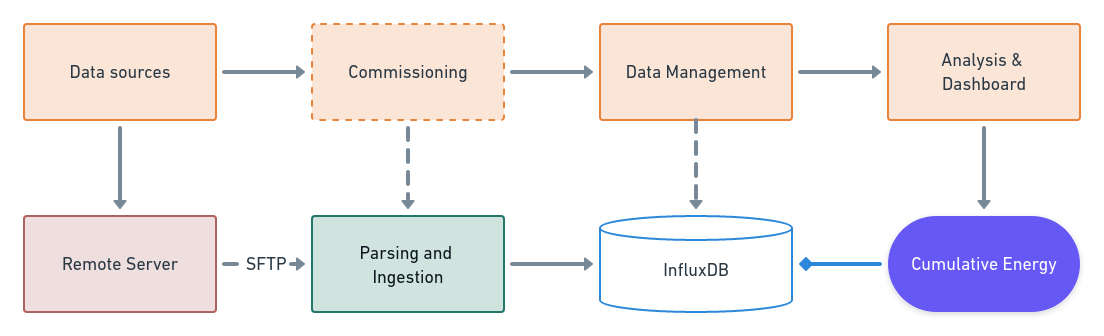
\includegraphics[width=0.8\textwidth]{vub/flowcharts/4_phases.png}
        \caption{Recap of \acs{VUB}'s project}
    \end{figure}
    Potential enhancements remain open, such as additional statistics
    to compare nodes and viable alarms on current, voltage and power \\
    factor values.

    \vspace*{\fill}
\end{frame}